\documentclass[14pt,a4paper,russian]{scrartcl}
% \documentclass[14pt,a4paper,oneside,russian,fontsize=14pt]{scrartcl}
\usepackage{mystyle}
\graphicspath{{images/}}

\begin{document}

\renewcommand{\onlyinsubfile}[1]{}
\renewcommand{\notinsubfile}[1]{#1}

% 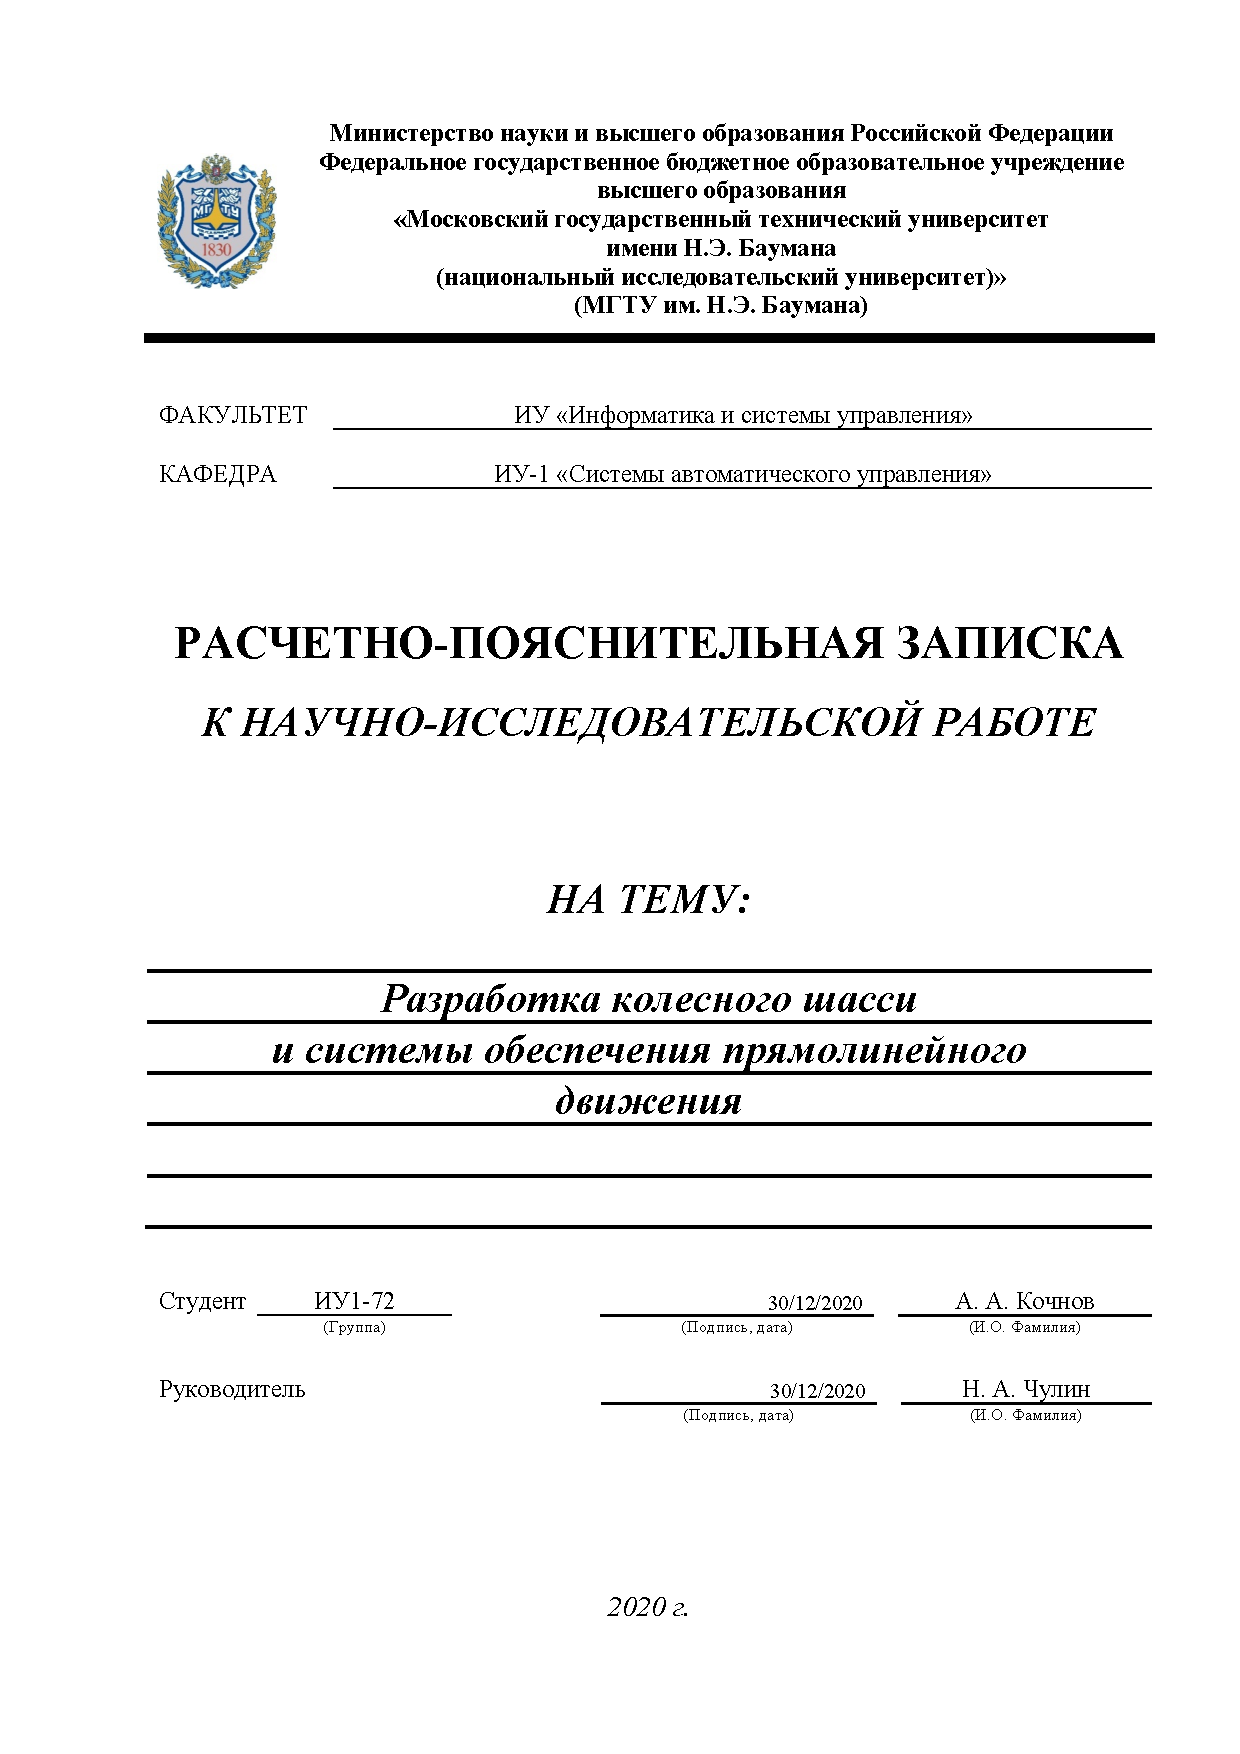
\includepdf[page={1}]{parts/titul}

\tableofcontents
\newpage

\section*{Вступление}
\addcontentsline{toc}{section}{Вступление}
Системы автоматического управления используются повсеместно. Основная 
их задача - поддерживать состояние системы в соответствии 
с некоторыми требованиями - движение по заданной траектории, поддержание температуры и т.д.

Одна из причин, почему контролируемая система начинает со временем
не соответствовать заданным условиям - это различные внешние воздействия. Например,
окружающая среда может похолодать, из-за чего автоматическая печь начнет остывать
быстрее. Или беспилотник начнет сносить в сторону боковой ветер. Кроме того, 
стабильности состояния может помешать несовершенство механизма, который управляется.
Например, люфт в механических передачах, неодинаковые параметры двигателей и т.д.

Для решения проблемы в систему управления вводится обратная связь и некоторый 
регулятор, чтобы компенсировать влияние помех. Поэтому ставятся задачи как чисто 
аналитического плана - синтез регулятора, так и технического - разработка
удачного ПО для непосредственного управления электромеханическими частями обьекта,
измерение необходимых параметров среды и состояния системы, предварительная обработка
и очистка сигнала, чтобы сделать его пригодным для анализа.

В данной НИР мы начинаем подготовительную работу для анализа работы и влияния
различных методов и приемов компенсации помех в работе подвижных объектов. 
Так как максимально продуктивным будет изучение на практике, необходимо разработать
подвижную мобильную платформу, способную перемещаться в пространстве в соответствии
с заданными командами, а также собирать и обрабатывать информацию о своем состоянии.
Выбран наземный вариант с перемещением в 2D-пространстве как наиболее простой вариант,
упрощающий реализацию но не основные принципы и идеи.

\newpage

\section*{Основная часть}
\addcontentsline{toc}{section}{Основная часть}
\subsection{Постановка задачи}
Как уже было указано, 
\newpage

\subsection{Практическая часть}
Основная задача на НИР этого семестра - создание платформы для отработки
приемов и методов управления. Процесс можно разделить на
несколько частей - сборка механической части, разработка ПО для микроконтроллера и 
разработка подобия управляющего терминала.

\subsubsection{Создание шасси}
В основе подвижного мобильного шасси лежит готовый комплект. Пример
представлен на рис. \ref{fig:shassis_dissassembled}. Он включает в себя пластиковую основу,
стойки-крепления, электрические двигатели постоянного тока с пластиковыми редукторами,
колёса с прорезиненным протектором (который, тем не менее, довольно хорошо скользит)
и дисками для тахометров.
\begin{figure}[h]
    \center{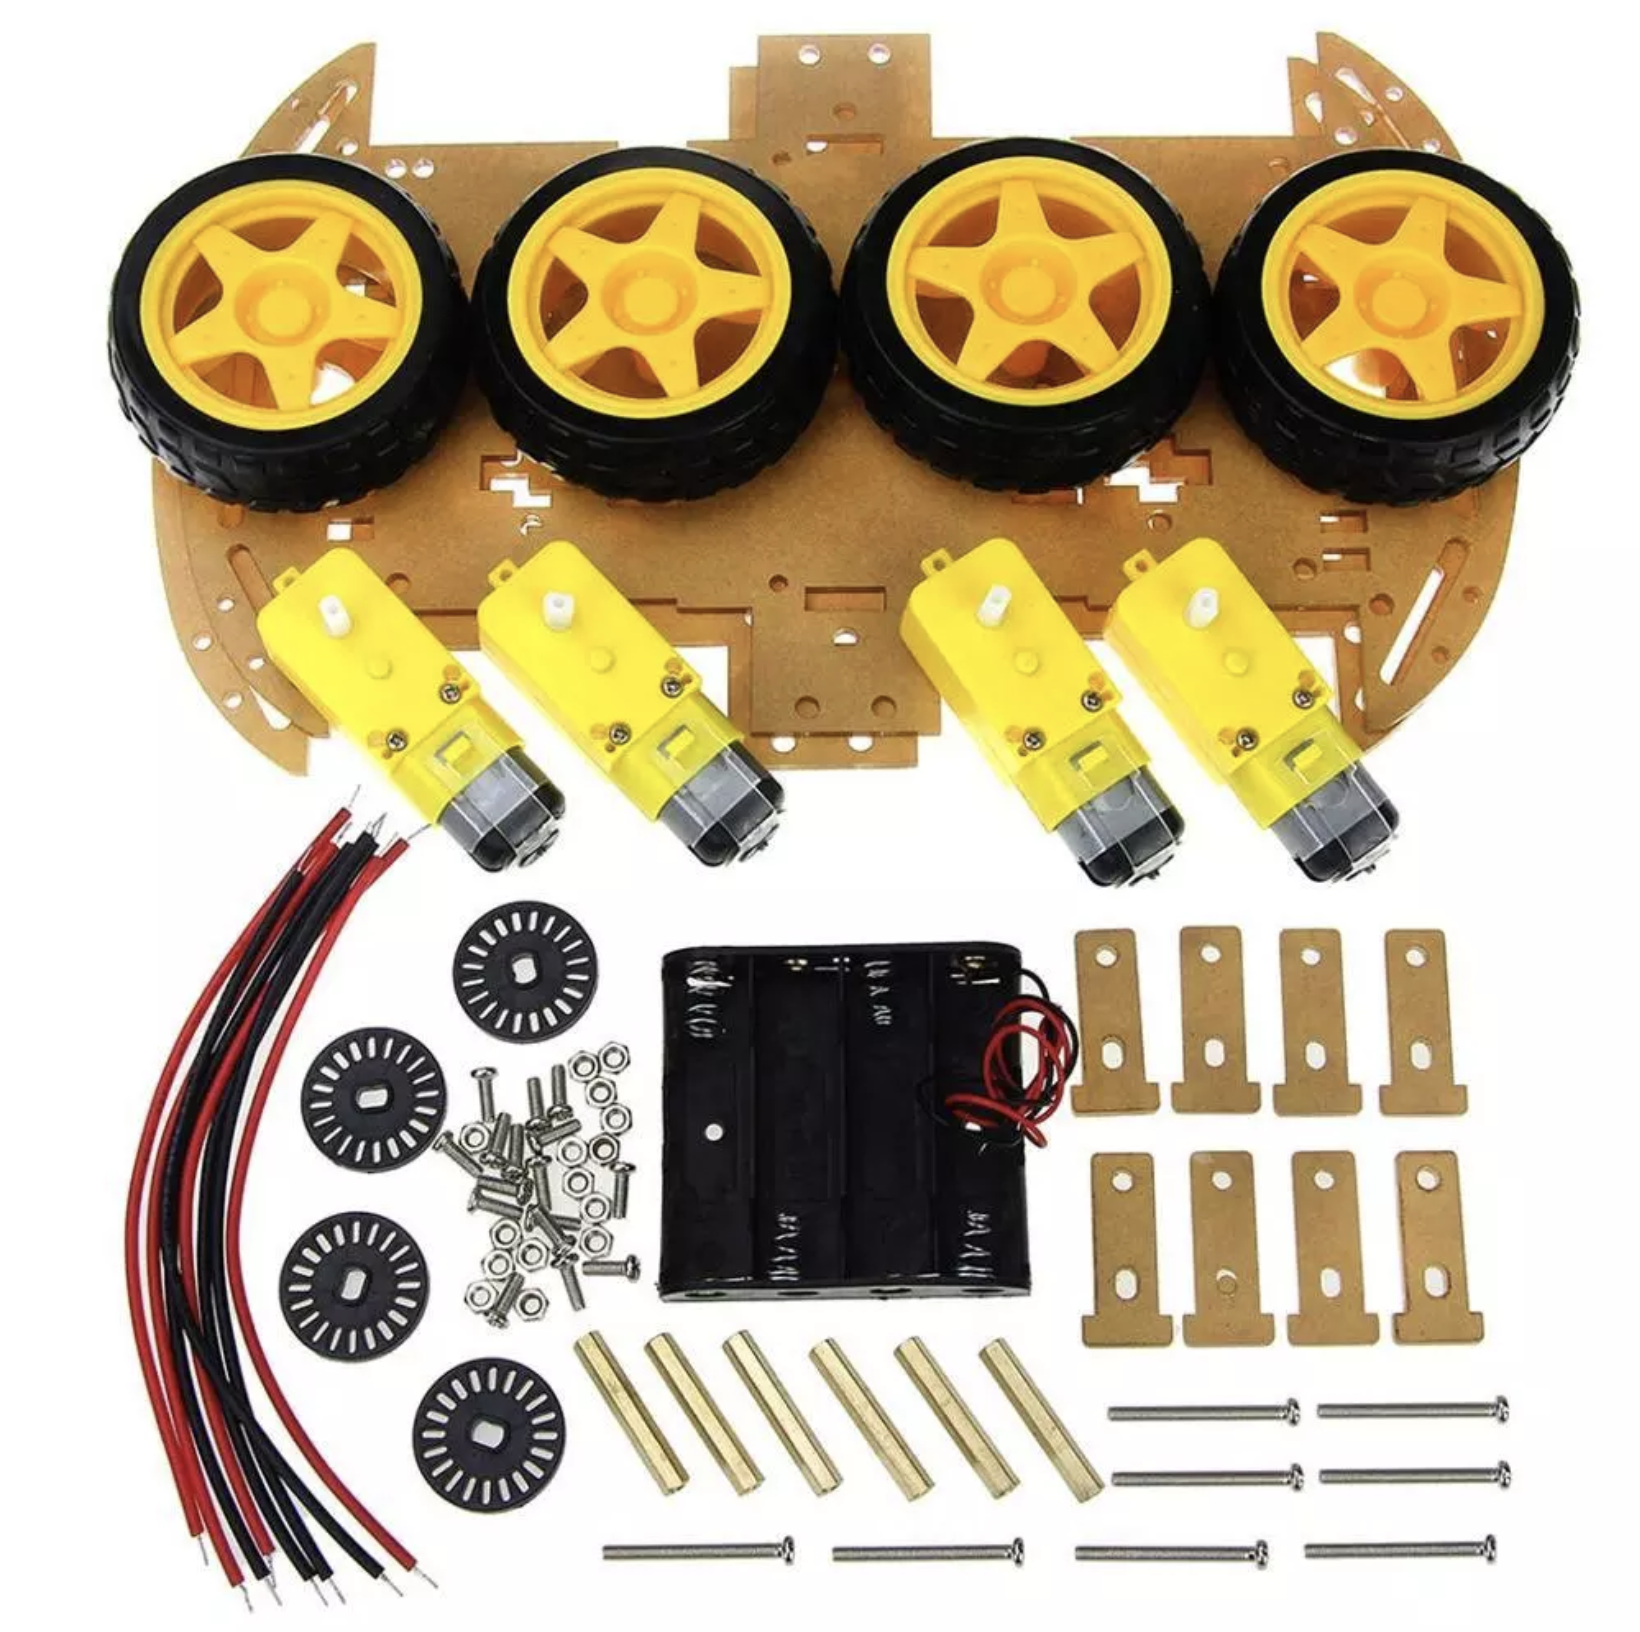
\includegraphics[width=0.8\linewidth]{shassis_dissassembled.png}}
    \caption{Основа шасси в разобранном виде}
    \label{fig:shassis_dissassembled}
\end{figure}

Как видно из фотографии, оригинальный комплект подразумевает наличие четырёх
ведущих колёс. Однако, как выяснилось в тестах, колеса начинают прокальзывать,
что вкупе с довольно неоднородными реальными характеристиками двигателей
превращало процесс движения шасси в довольно стохастичекий процесс. Поэтому
решено было оставить лишь два задних колеса, а для сохранения баланса
поставить вперёд ведомое колесо-подставку, которое дополнительно
легко вращается вокруг вертикальной оси, не препятствуя движению объекта. Заметим,
что массивные батареи также находятся сзади, что обеспечит колёсам хорошее
сцепление с поверхностью.

Комплект хороший, но этого недостаточно для поставленных задач. Далее шасси
необходимо дополнить электронными компонентами. 

Во-первых, необходим микроконтроллер. Рассматривались несколько вариантов:
\begin{itemize}
    \item Arduino (контроллеры семейства AVR серии ATmega, кроме Due)
    \begin{itemize}
        \item Uno (ATmega328 16 МГц, Flash 32Кб, RAM 2Кб, 14 IO pins)
        \item Mega 2560 (ATmega2560 16 МГц, Flash 256 Кб, RAM 8 Кб, 54 IO pins)
        \item Due (ARM AT91SAM3X8E 84 МГц, Flash 512 КБ, RAM 96 КБ, 54 IO pins)
        \item Pro mini (ATmega328 16 МГц, Flash 32 Кб, RAM 2 Кб, 14 IO pins)
    \end{itemize}
    \item STM32 (контроллеры семейства ARM)
    \begin{itemize}
        \item STM32F103C8T6 "Blue Pill" (Cortex M3 72Мгц, Flash 64Кб, RAM 32Кбб 37 IP pins)
    \end{itemize}
\end{itemize}
Наиболее популярный вариант - Arduino Uno. Обладает мощностями, достаточными
для решения задачи на начальном этапе, однако имеет достаточно большие размеры и
некоторые излишества, которые хороши для обучения работы с микроконтроллерами,
но не нужны в готовом устройстве. STM32 куда мощнее и быстрее, компактна
и вообще хороша во всём, кроме фреймфорков. Существуют удобные готовые подобия
RTOS (ОС реального времени), однако они довольно большие и занимают почти всю
доступную память данного контроллера начального уровня. Библиотеки более низкого
уровня сложныи требуют слишком много времени на освоение, что не предполагается
в данной задаче.

Итого, была выбрана плата Arduino Pro Mini, представленная на рис.\ref{fig:pro_mini}
\begin{figure}[h]
    \center{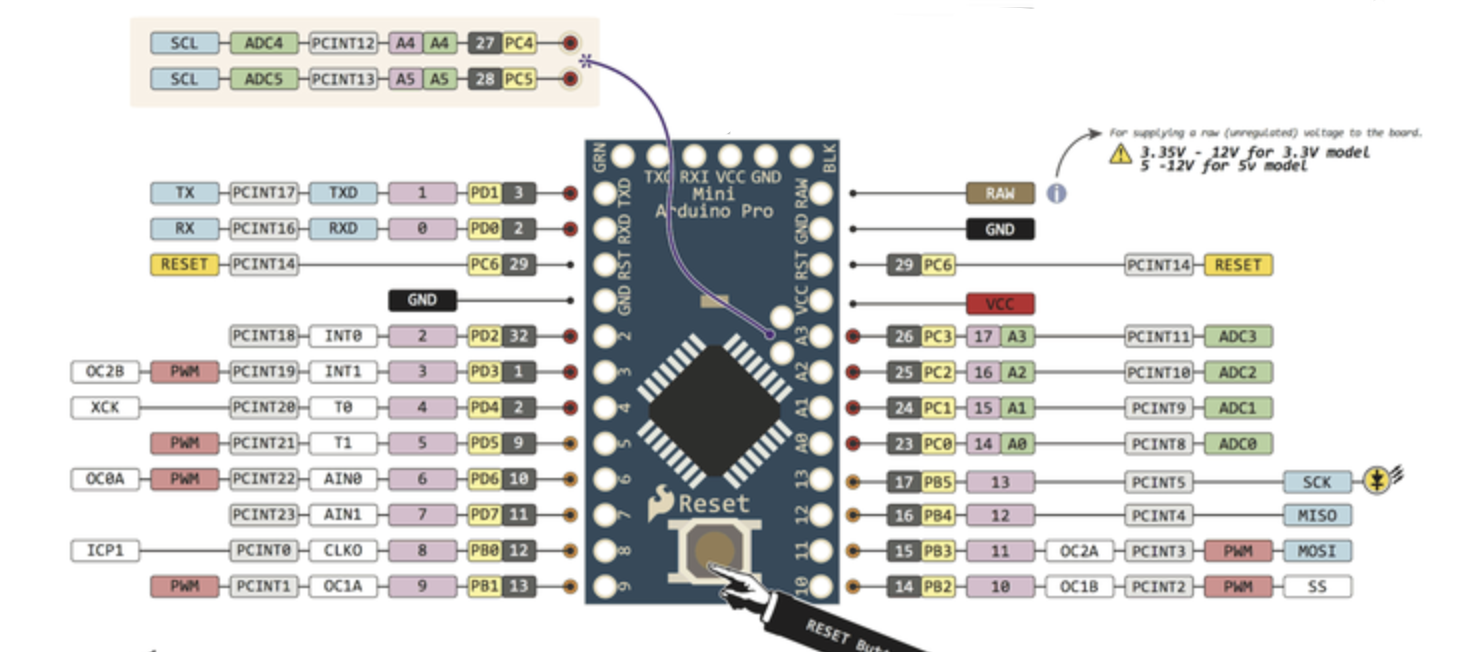
\includegraphics[width=1\linewidth]{pro_mini.png}}
    \caption{Arduino Pro mini со схемой распиновки}
    \label{fig:pro_mini}
\end{figure}

Основа любого мобильного шасси - это двигатели. В данной сборке их два - на каждое
колесо. Чтобы управлять направлением движения, необходимо менять полярность подключения
к источнику питания. Чтобы управлять скоростью (и усилием) вращения, используется
ШИМ-сигнал. Так как для двигателей необходимо высокое напряжение (7..8 В), большее,
чем требует контроллер (3.3 В), а также большой ток, двигатели подключаются
к так называемому драйверу электродвигателей. Он основан на Н-мосте, который позволяет
менять полярность подключения, а также транзисторных ключах, которые на основе ШИМ-сигнала
малого напряжения модулируют рабочее напряжение. В данной сборке использован драйвер
на базе микросхемы L298N, имеющий ровно два независимых канала. 
Представлен на рис.\ref{fig:motor_driver}.
\begin{figure}[h]
    \center{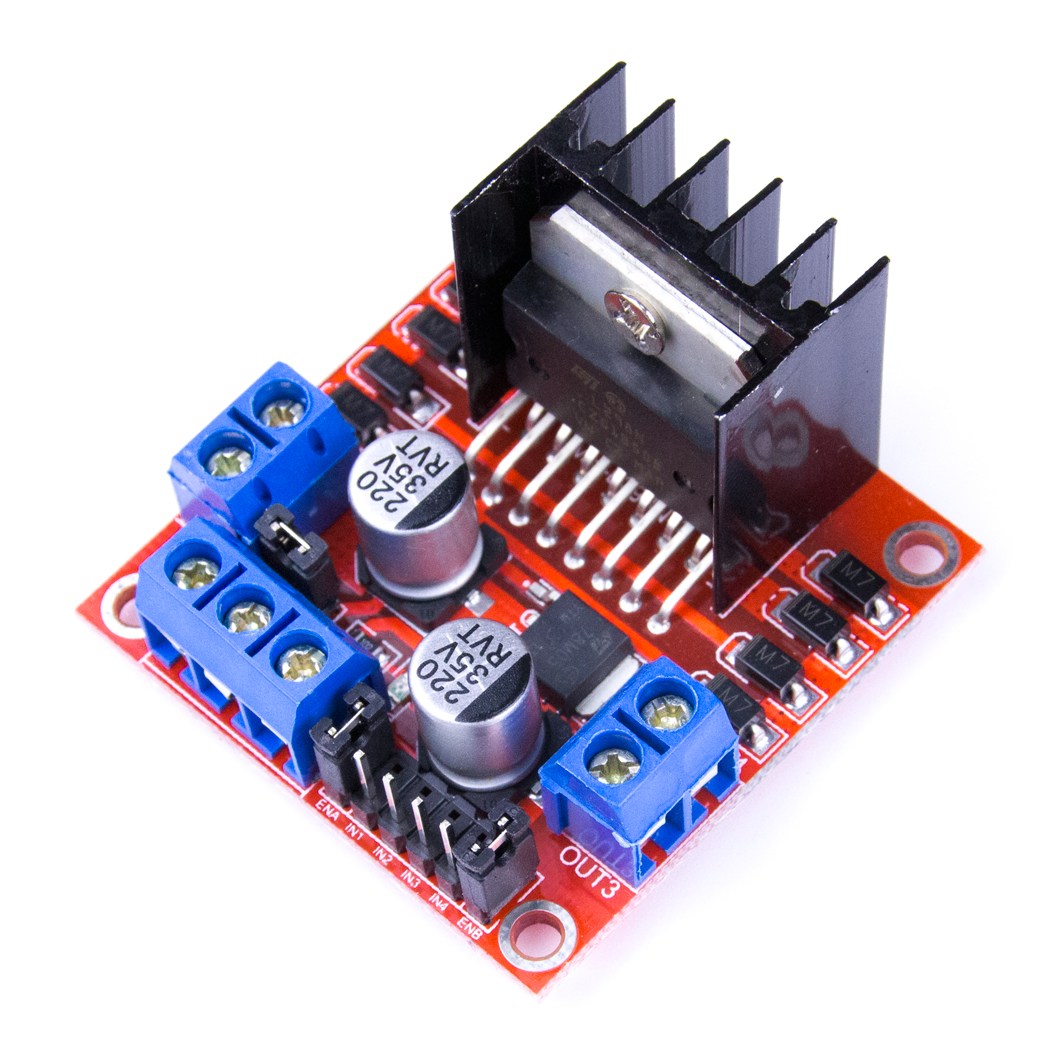
\includegraphics[width=0.6\linewidth]{motor_driver.png}}
    \caption{Драйвер электродвигателей L298N}
    \label{fig:motor_driver}
\end{figure}

Для определения состояния шасси для обеспечения обратной связи
необходимы датчики. Так как мы рассматриваем процесс движения, 
необходимо получать данные о пройденном пути, текущей скорости обьекта (как 
линейной, так и угловой), ускорения. 

Для контроля работы двигательной
подсистемы будем использовать оптические тахометры. Принцип действия использованных
оптических тахометров заключается в реакции на каждое прохождение препятствия
между светодиодом и оптическим приемником. Зная момент прохождения и количество
щелей в диске, можно довольно точно вычислять суммарный угол поворота колеса.
Проводя численное дифференциирование, можно получать угловые скорости (и даже
угловые ускорения) вращения каждого из колес. В итоге можно узнавать 
общую угловую (и линейную) теоретические скорость шасси, откуда компенсировать различия в параметрах (а
следовательно, и в реальной скорости вращения) двигателей, обеспечивая
прямолинейное движение. Приведён на рис.\ref(fig:encoder).
\begin{figure}[h]
    \center{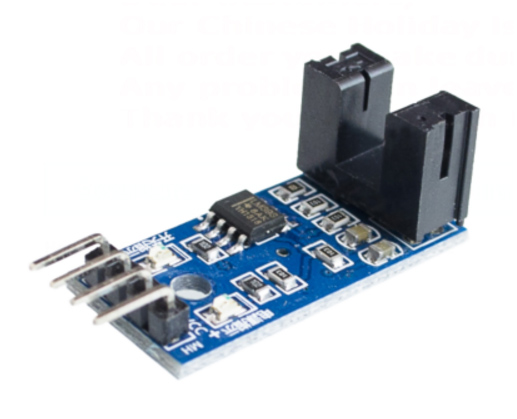
\includegraphics[width=0.6\linewidth]{encoder.jpg}}
    \caption{Оптический тахометр (энкодер)}
    \label{fig:encoder}
\end{figure}

Теоретические скорости - хорошая вещь. Но она получается в предположении
что колеса идеально сцепляются с повехностью без проскальзывания, 
а шасси не подвергаются внешним воздействиям и не упирается в препятствия.
Для получения данных о реальном состоянии движения используем связку 
гироскоп-акселерометр. Простейшие варианты поставляются в виде объединенной
платы, которая отличается не только весьма удовлетворительной точностью, но
и сверхнизкой стоимостью. Пример представлен на рис.\ref{fig:gyro_accel}.
\begin{figure}[h]
    \center{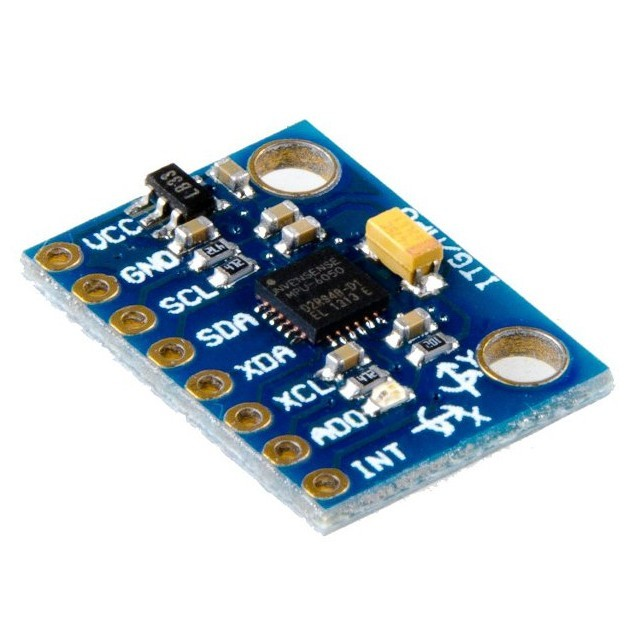
\includegraphics[width=0.6\linewidth]{gyro.jpg}}
    \caption{Гироскоп-акселерометр GY-521 (MPU-6050)}
    \label{fig:gyro_accel}
\end{figure}

Дополнительно можно использовать электронный датчик магнитного поля.
Вкупе модулем выше можно реализовать электронный компас, с помощью которого
измерять абсолютный угол поворота робота. Однако он подвержен помехам от 
двигателей, а также довольно сложен в реализации, поэтому в данной версии
не использовался. Выглядит очень схоже с платой гироскопа. Кроме того,
в роботы такого типа также ставятся ультразвуковые/инфракрасные датчики расстояния
или даже лидары. Однако в данной работе ставится задача лишь контроля
траектории шасси, поэтому эти устройства также не используются.

По заданию необходимо задавать роботу направление движения извне. Так как
шасси подвижное, необходима беспрроводная связь. Рассматривалось
и тестировалось несколько вариантов. Сначала предполагалось использование 
передатчика nRF24l01, позволяющего держать связь до 50м на открытом пространстве.
В этом случае команды не должны теряться в пределах помещения и доходить
быстро и надежно. Однако цепочка шасси <-радио-> приемник <-USB-> терминал
оказалась довольно сложной. Потому исходя из предположения небольших
размеров помещения для тестирования шасси использован простой bluetooth-передатчик,
держащий связь непосредственно с терминалом.

Терминал изначально предполагался физический. Однако имеющиеся джойстики
не предполагали высокого качества и точности выдаваемого сигнала, поэтому
эта идея была пропущена.

Дополнительно для схемы использовался понижающий преобразователь
напряжения для получения напряжения 5В для микроконтроллера и датчиков, 
Li-Ion батареи типоразмера 18650 и автономного вольтметра для 
визуального контроля состояния батарей.

Итоговый вариант сборки представлен на рис.\ref{fig:robocar_common_sight}.
\begin{figure}[h]
    % \center{\includegraphics[width=1\linewidth]{pic.png}}
    \caption{Итоговый вид мобильного робота}
    \label{fig:robocar_common_sight}
\end{figure}

\subsubsection{Разработка прошивки}
Второй важной частью разработки робота является написание ПО для микроконтроллера 
- прошивки. Она отвечает за обмен данными с командным терминалом,
расчет и подачу управляющих сигналов на двигатели, считывание данных
с сенсоров и расчет параметров движения для дальнейшей коррекции.

Так как разработка ведется под микроконтроллер Arduino, очевидным
решением является использование фирменного фреймворка, 
предоставляющего упрощенный и удобный интерфейс для взаимодействия
с железной составляющей проекта. Это вообще позволяет быстро писать 
короткие и лаконичные скрипты.

Однако прошлый опыт работы с такими проектами показал, что отлаживать 
работу программы на реальном роботе довольно сложно, трудоёмко и долго.
Кроме того, было желание разработать универсальную основу, в которую
в дальнейшем будет легко вносить дополнительную функциональность. Поэтому
решено было пойти сложным путём.

Для решения проблемы тестирования существует несколько вариантов. 
Первый - использовать встроенные возможности тестирования системы
программирования контроллеров PlatformIO. Она решает проблему регрессионного
тестирования - полной проверки старого функционала продукта после новых изменений.
Однако это не решало проблему абстрагирования от оборудования (а это важно, если
сбои могут быть именно в оборудовании, а не в коде, или же необходима
дополнительная информация о работе программы, которую не получить с железного
устройства). Поэтому решено было пойти путём, который применяется в реальных
продуктовых разработках программного обеспечения - создание копий функций
библиотеки Arduino, которые не используют реальное оборудование, а 
фиксируют факт вызова и возвращают заранее заданный результат. Процесс называется
автоматическим тестированием, а замены - mock-функциями (от англ. "mock" - шутка, насмешка).
В таком случае становится довольно просто создавать автоматические тесты,
которые проверяют правильность работы программы. Для эмуляции Arduino-вызовов
использовалась Open-Source библиотека ArduinoFake на основе google-test фреймфорка.

Так как в проекте предполагается несколько задач (обмен данными с терминалом,
управление двигателями, считывание данных тахометров и тд), возникает
вопрос обеспечения многозадачности. Микроконтроллеры такого класса 
как правило однопоточны. А стандартный фреймворк Arduino не предлагает
никаких решений этого вопроса, потому что предполагает лишь простые проекты.
Поэтому использовалась сторонняя библиотека LeOS2. Очевидно, что это никакая
не ОС, но обеспечение многозадачности - одна из их задач, поэтому название 
объяснимо. Эта библиотека работает на основе сторожевого таймера 
микроконтроллера (в отличие от первой версии, которая использует один из
таймеров ШИМ). Раз в 16 миллисекунд таймер срабатывает и вызывает прерывание,
которое перехватывается библиотекой, после чего по порядку запускается выполнение
тех заранее заданных функций ("задач"), которые должны сработать в этот момент
времени. Очевидно, что интевал исполнения задач должен быть кратен 16 миллисекундам.
Использование библиотеки с поддержкой псевдомногозадачности позволило
упростить основной сценарий работы программы и чётче разделить подзадачи.
Так как библиотека работает с аппаратным таймером в обход фреймворка Arduino,
для неё также была создана mock-версия. 

Таким образом, удалось полностью отвязать разработку основного 
программного кода от железной составляющей. Очевидно, это потребовало много
дополнительных усилий, однако уже на данном этапе это оказалось
очень полезно при разработке и сэкономило часть затраченного времени.

Для решения вопроса универсальности основы разработана компонентная
структура программы на основе классов языка C++, используемого при разработке.
UML-диаграмма представлена на рис.\ref{fig:firmware_uml}. Частично
применена идея MVC-архитектуры (модель-контроллер-интерфейс).
\begin{figure}[h]
    \center{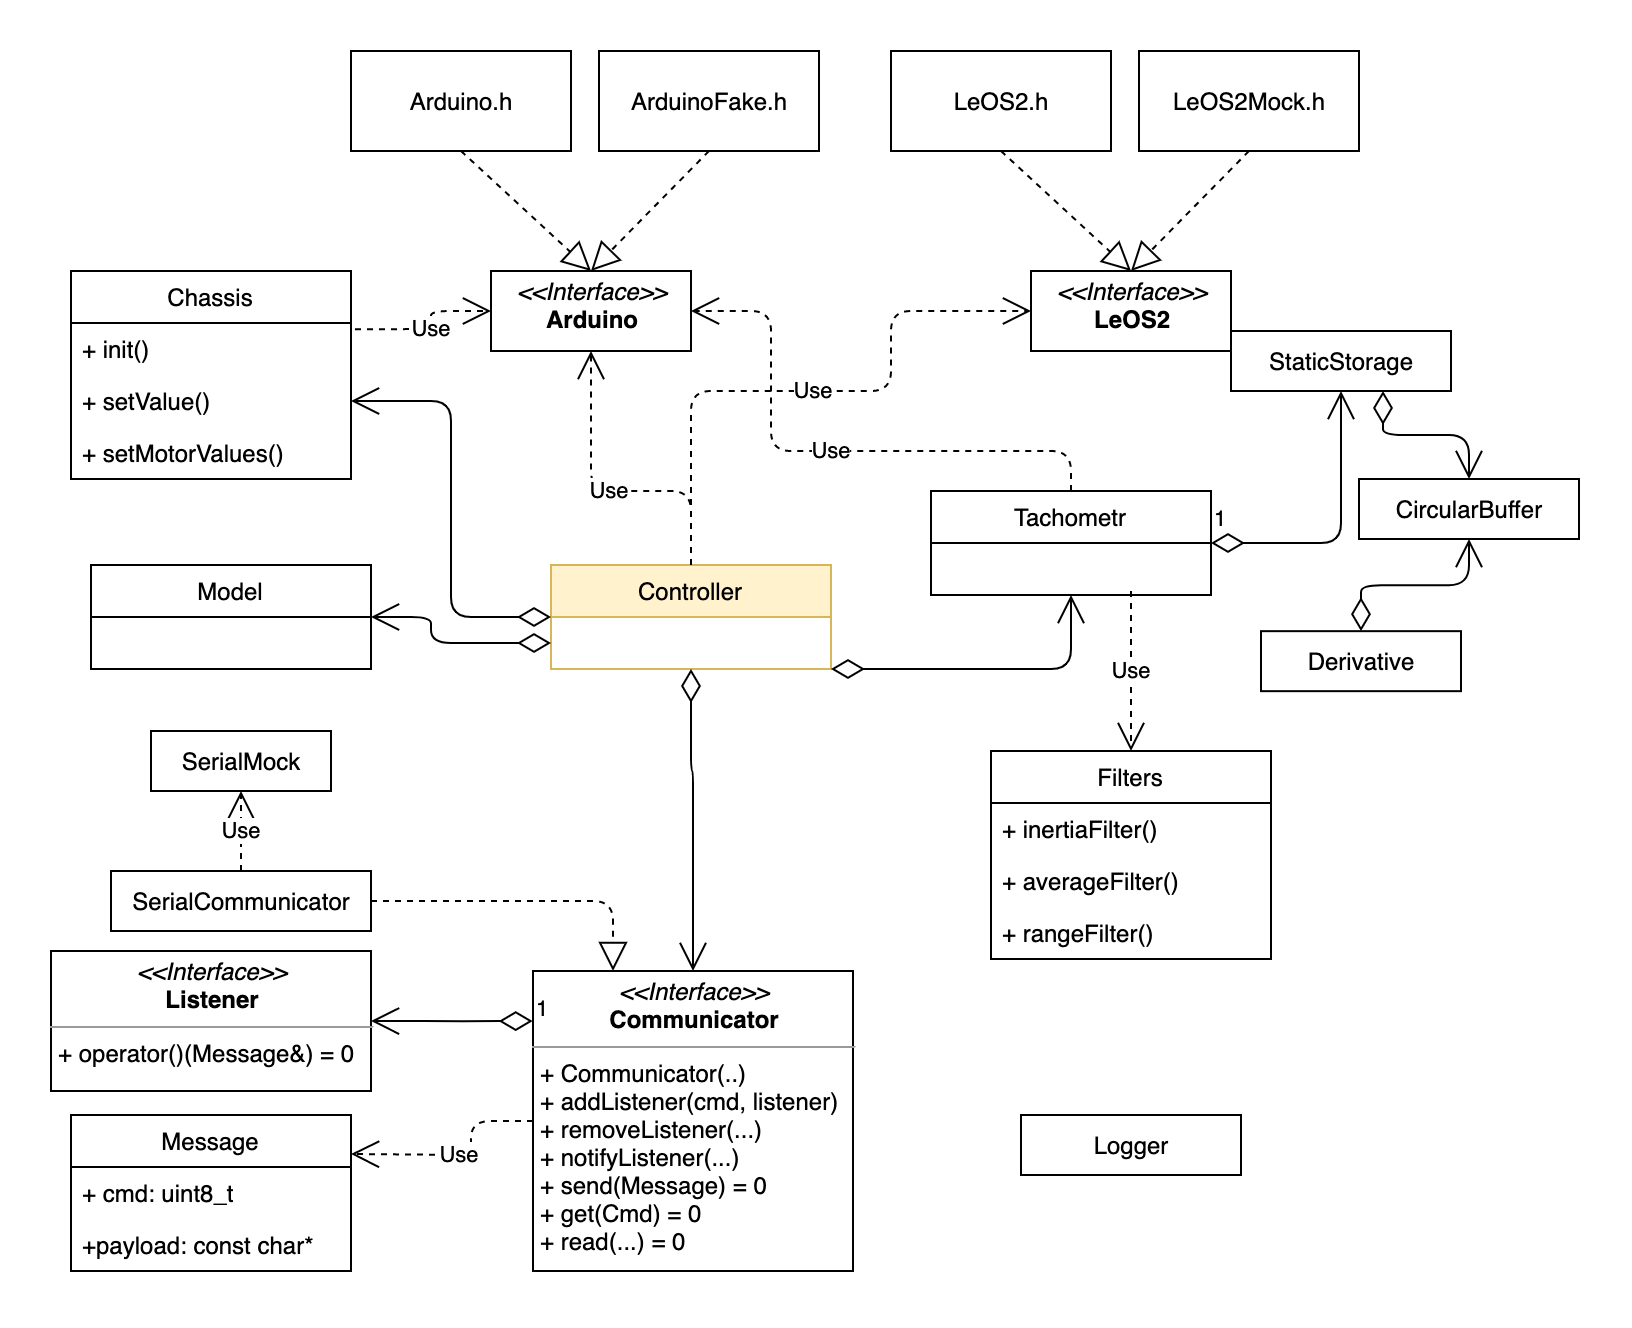
\includegraphics[width=1\linewidth]{firmware_2.png}}
    \caption{UML-диаграмма блоков прошивки}
    \label{fig:firmware_uml}
\end{figure}

Центральным модулем является Controller. Он отвечает за инициализацию
и сбор воедино всех компонентов. Model отвечает за хранение данных о состоянии
шасси (в идеале должно и вычислять, но на данным момент этим занимается Controller).
Chassis принимает на вход требуемые параметры движения двигателей (в 
различных шкалах), преобразует в необходимый вид и подает на двигатели.

Tachometr отвечает за обработку аппаратных прерываний на проход щели мимо детектора
и вычисление пройденного расстояния и текущей скорости. Данные хранятся в зацикленном
буфере CircularBuffer. Из-за особенностей языка и требований к обработчикам аппаратных
прерываний возникла необходимость в создании статического хранилища данных
StaticStorage, аггрегирующий данные, необходимые для работы обработчика прерывания
и расчета скоростей и расстояний.

Для связи разработана система классов. Основная идея - абстрагировать
работу с обменом данных до единого интерфейса. Сейчас его 
реализует только класс для работы с Serial-протоколом, но в дальнейшем
не исключается возможность работы с передатчиками, такими как nRF24l01. 
Как видно из схемы, для SerialCommunicator сделана mock-эмуляция 
Serial-подбиблиотеки Адуино. Благодаря
использованию интерфейса основной код не нужно будет менять. 
Кроме того, применен паттерн "Слушатель". Основная идея следующая. При
инициализации системы регистрируются несколько типов команд со своими кодами 
(например, для подачи управления, для обновления конфигурации, для
подачи звукового сигнала, поворота камеры и т.д.). Для каждой команды
регистрируются один или несколько "слушателей"\  - функций, которые должны
обработать новое сообщение такого типа, когда оно придёт извне. Слушателей
можно добавлять, удалять, вызывать. Для создания своего слушателя достаточно
наследовать интерфейс Listener и реализовать функцию operator(). 

Реализована поддержка динамической конфигурации. Константы, которые могут
быть изменены без перезагрузки системы - изменяемы. Достаточно прислать
с терминала команду с названием переменной и новым значением. Например,
можно изменять константы в фильтрах, включать/отключать некоторые и сразу же
наблюдать изменение поведения шасси.

В главном скрипте инициализируется сам контроллер и запускаются несколько задач:
\begin{itemize}
    \item проверка "почты" - наличия данных во входном serial-буфере. Если данные
    есть - вызываем всех слушателей на эти данные;
    \item расчет текущих скорости и ускорения по данным тахометра;
    \item заготовка для регулятора - коррекции траектории,
\end{itemize}
а также несколько входящих команд:
\begin{itemize}
    \item получения нового значения желаемого направления движения
    \item получение нового значения желаемой скорость движения
    \item обновление конфигурационных параметров
    \item "ping" - ответ на проверочное значение от терминала (жив ли робот).
\end{itemize}

Работа с гироскопом и акселерометром на данный момент не реализована.

\subsubsection{Определение параметров движения робота}
Как уже упоминалось выше, на данный момент единственным источником данных
о состоянии шасси для обратной связи является тахометр. Устройство максимально просто работает.
На ось колеса ставится диск с прорезями известного числа, расположенные через
равные интервалы. Диск просвечивается светодиодом. Как только на пути света оказывается
щель в диске, первый попадает в фоторезистор, после чего генерируется электрический
сигнал, вызывающий аппаратное прерывание в контроллере. Программа регистрирует
время срабатывания датчика (в микросекундах). На данном устройстве диск имеет 23 щели,
откуда легко понять, что датчик будет срабатывать довольно часто, оттуда и микросекунды.

В данный момент для простоты работы расчёт скоростей и расстояния происходит на каждое
срабатывание датчика, но в дальнейшем планируется связать этот процесс с 
коррекцией, чтобы оптимизировать вычислительные затраты. Прерывание должно работать быстро.

Опишем процесс расчёта пройденного расстояния и скорости колеса. Для каждого прерывания
записывается время в микросекундах, прошедшее с момента последнего срабатывания.
Затем инкрементируется текущая координата вдоль пути и расставляются необходимые
служебные флаги. Затем через некоторое время начинается расчет скорости. Сначала выполняется
расчет производной с новым значением путевой координаты на основе сохраненных ранее
предыдущих значений. Затем применяются различные фильтры. В данный момент включены: бегущее
среднее, оконный усредняющий фильтр. Их параметры доступны для изменения в режиме
реального времени. Затем данные сохраняются в модель и становятся доступными для регулятора. 
Вообще структура программы позволяет легко вычислять и ускорение, просто добавив
еще один модуль производной. Однако, как увидим далее, в текущей реализации это
довольно бессмыссленно из-за низкой точности.

Так как сигнал значений скорости очень важен, довольно много времени
уделено отработке алгоритмов его обработки. Анализ проводился в Matlab 
на основе реальных данных, собранных с шасси. Для этого прошивка была изменена
таким образом, чтобы данные с тахометра печатались в serial-порт, откуда попадали в текстовый файл.
Оттуда с помощью регулярных выражений данные преобразовывались в массив Matlab и вставлялись в скрипт.
Для лучшего тестирования алгоритмов в выборке попадали моменты как с равномерной работой двигателей,
так и резкие остановки/разгоны, а также изменения скорости между уровнями. 
Такая подготовка предоставила широчайшие возможности для анализа.

\section*{Заключение}
\addcontentsline{toc}{section}{Заключение}

\newpage


\newpage
\end{document}